\documentclass[conference]{IEEEtran}
\IEEEoverridecommandlockouts
% The preceding line is only needed to identify funding in the first footnote. If that is unneeded, please comment it out.
\usepackage{cite}
\usepackage{amsmath,amssymb,amsfonts}
\usepackage{algorithmic}
\usepackage{graphicx}
\usepackage{textcomp}
\usepackage{xcolor}
\usepackage{adjustbox}
\usepackage{hyperref}
\def\UrlBreaks{\do\/\do-}
\def\BibTeX{{\rm B\kern-.05em{\sc i\kern-.025em b}\kern-.08em
    T\kern-.1667em\lower.7ex\hbox{E}\kern-.125emX}}
\begin{document}

\title{Análise e Comparação do Algoritmo de Hash Argon2\\
}

\author{\IEEEauthorblockN{Nelson Vieira}
\IEEEauthorblockA{\textit{Faculdade de Ciências Exatas e da Engenharia} \\
\textit{Universidade da Madeira}\\
Funchal, Portugal \\
2080511@student.uma.pt}
}

\maketitle

\begin{abstract}
Este artigo serve como uma análise sobre o algoritmo de \textit{hash} Argon2, será realizada 
uma análise do algoritmo, tentando perceber a necessidade da sua criação, os pontos 
fortes e os pontos fracos, e o que este algoritmo oferece em relação a outros 
algoritmos de \textit{hash} já existentes. Sobretudo este artigo procura responder as 
seguintes questões: porquê que este algoritmo está a ser recomendado e será que 
devemos substituir os algoritmos que estão em uso por este?
\end{abstract}

\begin{IEEEkeywords}
Argon2, criptografia, algoritmo de \textit{hash}
\end{IEEEkeywords}

\section{Introdução}
\IEEEPARstart{A}{}s palavras-passe, apesar de todas as suas desvantagens, permanecem a forma 
principal de autenticação em vários serviços da Web. 
As palavras-passe são geralmente armazenadas num formato \textit{hash} na base de dados 
de um servidor \cite{argon2spec}. Uma função de \textit{hash} criptográfica é um procedimento matemático que 
converte dados de qualquer tamanho, podemos chamar estes dados de "mensagem", numa 
matriz de bits de tamanho fixo, o valor de \textit{hash}. É uma função unidirecional, o que 
significa que inverter ou reverter a computação é quase impossível. A única maneira 
de encontrar uma mensagem que gera um \textit{hash} específico é tentar uma pesquisa de força 
bruta de todas as entradas em potencial para ver se alguma delas fornece uma correspondência 
ou usar uma rainbow table de \textit{hashes} correspondentes. A criptografia moderna depende 
muito de funções de \textit{hash} criptográficas.
Bases de dados são bastante frequentemente capturados 
por atacantes, que aplicam ataques de dicionário, já que as palavras-passe 
tendem a ter entropia baixa. Os designers de protocolo usam um número de 
truques para mitigar esses problemas. 
Uma função \textit{hash} criptográfica deve ser determinística, o que significa que deve sempre produzir o 
mesmo \textit{hash} para a mesma mensagem. Também deve ter geralmente as seguintes características: 

\begin{itemize}
\item O valor de \textit{hash} para cada mensagem fornecida pode ser calculado rapidamente;
\item É impossível criar uma mensagem que retorne um determinado valor de \textit{hash} (ou seja, reverter o processo 
que gerou o valor de \textit{hash} fornecido);
\item É impossível encontrar duas mensagens que tenham o mesmo valor de \textit{hash};
\item Uma pequena alteração numa mensagem deve fazer com que o valor de \textit{hash} mude tão drasticamente 
que o novo valor de \textit{hash} pareça não relacionado ao valor de \textit{hash} anterior (efeito de avalanche).
\end{itemize} \cite{al2011cryptographic}

Organizações e programadores recebem muitas novas opções no uso de mecanismos criptográficos. 
Escolhas inadequadas podem resultar numa ilusão de segurança, mas pouca ou nenhuma segurança 
real para o protocolo ou aplicação.
A partir do final dos anos 70, as 
palavras-passe passaram a ser \textit{hashed} com um valor de \textit{salt} aleatório para evitar a 
deteção de palavras-passe idênticas em diferentes utilizadores e serviços. Os 
cálculos de função de \textit{hash}, que se tornaram mais rápidos e mais rápidos 
devido à lei de Moore, foram chamados várias vezes para aumentar o custo 
de tentativas de palavra-passe para o atacante. \cite{argon2spec}

Muitas aplicações de segurança da informação usam funções de \textit{hash} criptográfico, incluindo 
assinaturas digitais, códigos de autenticação de mensagem e outras formas de autenticação. 
Também podem ser usados como funções de \textit{hash} regulares, indexação de dados em tabelas de \textit{hash}, 
fingerprint, deteção de dados duplicados e como 
checksums para detetar corrupção de dados. Os valores de \textit{hash} criptográficos são frequentemente 
referidos como fingerprints, checksums ou simplesmente valores de \textit{hash} em contextos de 
segurança de sistemas de informação, apesar de todas essas terminologias referirem-se a funções mais 
genéricas com atributos e objetivos bastante distintos. \cite{hashwiki}

O Argon2 é um algoritmo de \textit{hash} criptográfico que tem como objetivo resolver 
os problemas atuais do processo de \textit{hashing}, criado por Alex Biryukov, 
Daniel Dinu e Dmitry Khovratovich da Universidade de Luxemburgo. O Argon2 
possui 6 parâmetros de entrada: \textit{password}, \textit{salt}, custo de memória (o uso de 
memória do algoritmo), custo de tempo (o tempo de execução do algoritmo e o 
número de iterações), fator paralelismo (o número de fios paralelos), 
comprimento da \textit{hash}.

Este algoritmo de \textit{hash} criptográfico é uma \textit{key derivation function} (KDF) que foi 
selecionada como o vencedor da Password Hashing Competition \cite{phc} em 2015, 
ganhou esta competição de entre 24 algoritmos. Para além de ganhar esta 
competição também foi aceite como um standard RFC 9106 \cite{rfc9106} em 2021.


\section{Razão da Criação do Algoritmo}

\subsection{Os esquemas existentes de \textit{hashing} e os seus problemas}

A solução trivial para \textit{hash} de palavra-passe é uma função de \textit{hash} digitada como o HMAC, 
mas esta solução requer o uso de chaves secretas. Se o designer de protocolo 
preferir \textit{hashing} sem chaves secretas para evitar todos os problemas com geração, 
armazenamento e atualização de chaves, ele tem poucas alternativas: 
o modo genérico PBKDF2, o bcrypt baseado no Blowfish, e scrypt. Entre esses, 
apenas scrypt visa a alta memória, mas a instabilidade de uma troca de tempo 
trivial permite implementações compactas com o mesmo custo de energia. 
O design de uma função memory-hard provou ser um problema difícil. Desde o 
início dos anos 80, sabe-se que muitos problemas criptográficos que 
aparentemente exigem memória grande, na verdade, permitem uma troca de 
tempo de memória, onde o atacante pode negociar memória por tempo e 
fazer o seu trabalho no hardware rápido com memória baixa. Em aplicação aos 
esquemas de \textit{hash} de palavra-passe, isso significa que os crackers de palavra-passe ainda podem 
ser implementados num hardware dedicado, mesmo que por algum custo adicional. 
Outro problema com os esquemas existentes é a sua complexidade. O mesmo scrypt 
chama uma pilha de sub-processos, cuja razão de design não foi totalmente motivada. 
É difícil analisar e, além disso, difícil conseguir confiança. Finalmente, 
não é flexível em separar o tempo e os custos de memória. Ao mesmo tempo, 
a história das competições criptográficas demonstrou que os projetos mais 
seguros vêm com simplicidade, onde cada elemento é bem motivado e um 
criptoanalista tem apenas poucos pontos de entrada. 

A Password Hashing Competition, que começou em 2014, destacou os seguintes problemas: 
\begin{itemize}
\item O que acontece se o endereçamento de memória for independente do input ou 
dependente do input, ou híbrido? 
\item O primeiro tipo de esquemas, onde o local de leitura da memória é conhecida 
com antecedência, é imediatamente vulnerável aos ataques de time-space tradeoff, 
já que um atacante pode pré-computar o bloco ausente no momento em que é necessário. 
Por sua vez, os esquemas dependentes do input são vulneráveis a ataques side-channel, 
como as informações de tempo permitem uma pesquisa de palavra-passe muito mais rápida. 
\item É melhor encher a memória mas sofrer de compensações de espaço-tempo, ou fazer 
mais passes pela memória para ser mais robusto? Esta questão foi bastante difícil 
de responder devido à ausência de ferramentas de tradeoff genéricas, 
que analisaria a segurança contra ataques de troca e a ausência de métrica 
unificada para medir os custos do adverário. Como os endereços independentes do 
input devem ser computados? Várias opções aparentemente seguras foram atacadas.
\item Quão grande bloco de memória único deve ser? Ler blocos menores colocados 
aleatóriamente é mais lento (em ciclos por byte) devido ao princípio da 
localidade espacial do cache do CPU. Por sua vez, blocos maiores são dificeis 
de processar devido ao número limitado de registradores longos. Se o bloco 
for grande, como escolher a função de compactação interna? Deve ser criptograficamente 
seguro ou mais leve, fornecendo apenas uma mistura básica das entradas? 
Muitos candidatos simplesmente propuseram uma construção iterativa e argumentavam 
contra transformações criptograficamente fortes. 
\item Como explorar várias cores das CPUs modernas, quando estiverem disponíveis? 
Paralelizar chamadas para a função de \textit{hashing} com qualquer interação está sujeita 
a ataques tradicionais simples.
\end{itemize} \cite{argon2spec}

\subsection{Solução proposta pelo Argon2 para os problemas de esquemas existentes}

O Argon2 é uma função memory-hard. É um design simplificado. Visa a maior taxa de 
enchimento de memória e uso efetivo de várias unidades de computação, 
enquanto ainda fornece defesa contra ataques de trade-off. O Argon2 é otimizado 
para a arquitetura X86 e explora a organização de cache e memória dos recentes 
processadores Intel e AMD. O Argon2 tem uma variante principal, Argon2id e 
duas variantes suplementares, Argon2d e Argon2i. O Argon2d usa acesso à memória 
dependente de dados, o que o torna adequado para criptomoedas e aplicações sem ameaças 
de ataques de temporização \textit{side-channel}. O Argon2i usa acesso à memória 
independente de dados, que é preferido para \textit{hash} de palavra-passe e derivação de 
chave baseada em palavra-passe. O Argon2id funciona como Argon2i para a primeira metade 
da primeira passagem sobre a memória e como Argon2d para o resto, 
fornecendo assim a proteção de ataques \textit{side-channel} e poupança de 
força bruta devido a trade-offs de tempo de memória. O Argon2i faz mais passes pela memória 
para proteger de ataques de trade-off. \cite{rfc9106}

Argon2 é um tipo de computação memory-hard em que, como paradigma genérico, 
consiste no seguinte: cada tarefa é amalgamada com um determinado procedimento que 
requer acesso intensivo à RAM tanto em termos de tamanho quanto (muito importante) 
largura de banda, de modo que a transferência de computação para GPU, FPGA e até mesmo 
ASIC (application-specific integrated circuit) traz pouca ou nenhuma redução de custos. 
Esquemas criptográficos que são executados neste contexto tornam-se igualitários no 
sentido de que os utilizadores e os invasores são iguais nas condições de relação de 
desempenho de preços. \cite{biryukov2016egalitarian}

% Argon2 tem os seguintes parâmetros de entrada:

% \begin{itemize}
% \item Cadeia de mensagens P, que é uma senha para aplicações de hash de senha. 
% Deve ter um comprimento não superior a $2^{32}-1$ bytes.
% \item Nonce S, que é um salt para aplicações de hash de senha. Isto deve ter um 
% comprimento não superior a $2^{32}-1$ bytes. 16 bytes é recomendado para hash de senha. 
% O sal deve ser exclusivo para cada senha.
% \item O grau de paralelismo p determina quantos independentes (mas sincronizando) 
% cadeias computacionais (pistas) podem ser executadas. Isso deve seja um valor inteiro 
% de 1 a $2^{24}-1$.
% \item O tamanho da tag T deve ser um número inteiro de bytes de 4 a $2^{32}-1$.
% \item O tamanho da memória m DEVE ser um número inteiro de kibibytes de 8*p a $2^{32}-1$. 
% O número real de blocos é m', que é m arredondado até o múltiplo mais próximo de 4*p.
% \item Número de passagens t (usado para ajustar o tempo de execução independentemente o 
% tamanho da memória) DEVE ser um número inteiro de 1 a $2^{32}-1$.
% \item Número da versão v DEVE ser um byte 0x13.
% \item O valor secreto K é OPCIONAL. Se usado, DEVE ter um comprimento não maior que $2^{32}-1$ bytes.
% \item Os dados associados X são OPCIONAIS. Se usado, DEVE ter um comprimento não maior que $2^{32}-1$ bytes.
% \item Digite y DEVE ser 0 para Argon2d, 1 para Argon2i ou 2 para Argon2id.
% \end{itemize}

Argon2 tem dois tipos de entradas: entradas primárias e entradas secundárias, ou parâmetros. 
As entradas primárias são a mensagem $P$ e o nonce $S$, que são palavra-passe e \textit{salt}, respectivamente, para o 
\textit{hash} de palavra-passe. As entradas primárias devem sempre ser fornecidas pelo usuário de forma que
\begin{itemize}
\item A mensagem $P$ pode ter qualquer tamanho de $0$ a $2^{32}-1$ bytes;
\item Nonce $S$ pode ter qualquer tamanho de $8$ a $2^{32}-1$ bytes (16 bytes é recomendado para \textit{hash} de palavra-passe).
\end{itemize}
As entradas secundárias têm as seguintes restrições:
\begin{itemize}
\item O grau de paralelismo $p$ determina quantas cadeias computacionais independentes (mas sincronizadas) 
podem ser executadas. Pode levar qualquer valor inteiro de 1 a $2^{24}-1$.
\item O tamanho da tag $\tau$ pode ser qualquer número inteiro de bytes de 4 a $2^{32}-1$.
\item O tamanho da memória $m$ pode ser qualquer número inteiro de kilobytes de $8p$ a $2^{32}-1$. O número 
real de blocos é $m'$, que é $m$ arredondado para o múltiplo mais próximo de $4p$.
\item Número de iterações $t$ (usado para ajustar o tempo de execução independentemente do tamanho da memória) 
pode ser qualquer número inteiro de 1 a $2^{32}-1$;
\item O número da versão $v$ é um byte $0x13$;
\item O valor secreto $K$ (serve como chave, se necessário, mas não assumimos nenhum uso de chave por padrão) 
pode ter qualquer tamanho de $0$ a $2^{32}-1$ bytes.
\item Os dados associados $X$ podem ter qualquer tamanho de $0$ a $2^{32}-1$ bytes.
\item Digito $y$ de Argon2: 0 para Argon2d, 1 para Argon2i, 2 para Argon2id.
\end{itemize}

\begin{figure}[ht]
\centering
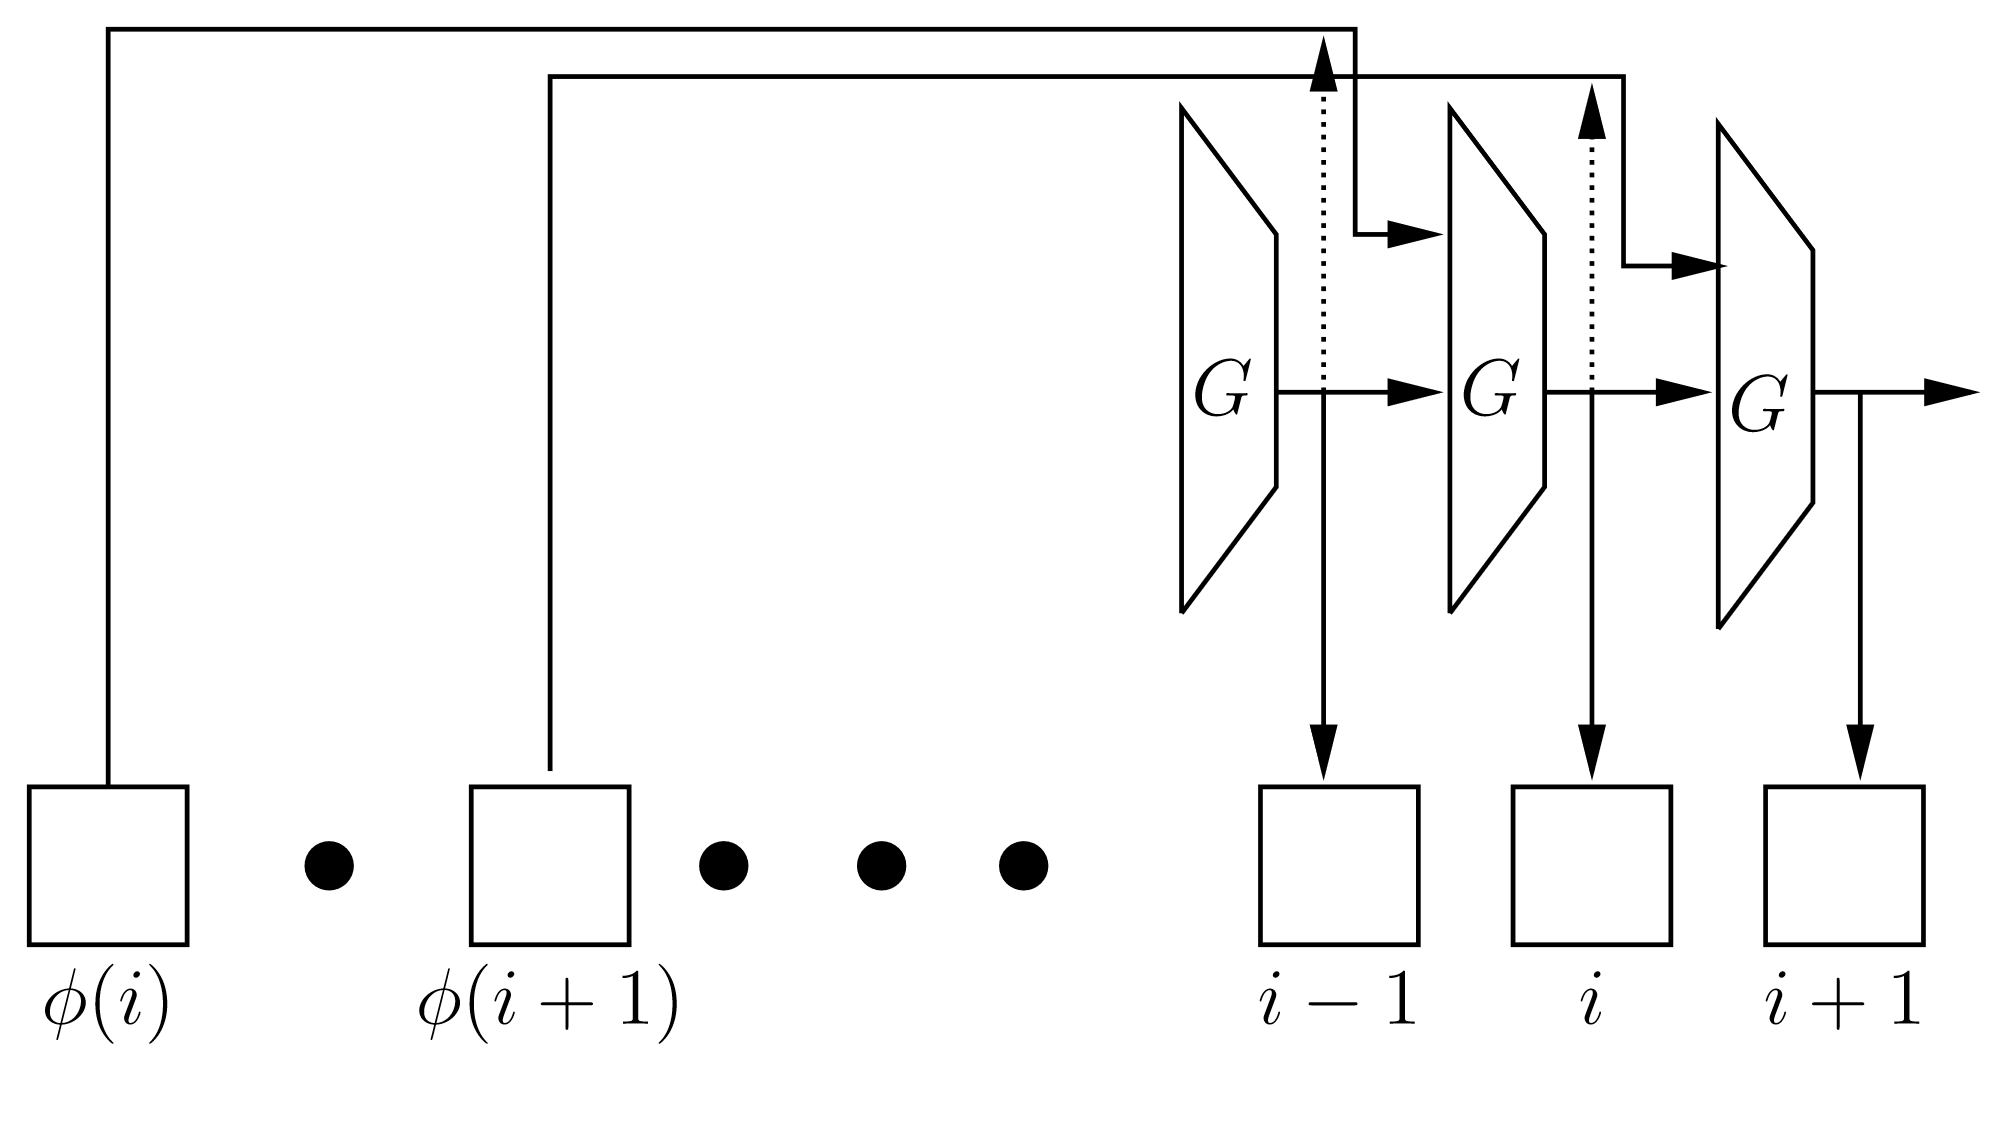
\includegraphics[scale=0.1]{assets/argon2-no-parallelism.png}
\caption{Argon2 em modo de operação sem paralelismo. }\label{fig:generic}
\end{figure}

O modo de operação do Argon2 é bastante simples quando nenhum paralelismo é usado: 
a função ${G}$ é iterada $m$ vezes. Na etapa $i$ um bloco com índice $\phi(i)<i$ é retirado 
da memória como podemos ver na figura \ref{fig:generic}, onde $\phi(i)$ é determinado pelo 
bloco anterior em Argon2D, ou é um valor fixo em Argon2i.

\begin{figure}[ht]
\centering
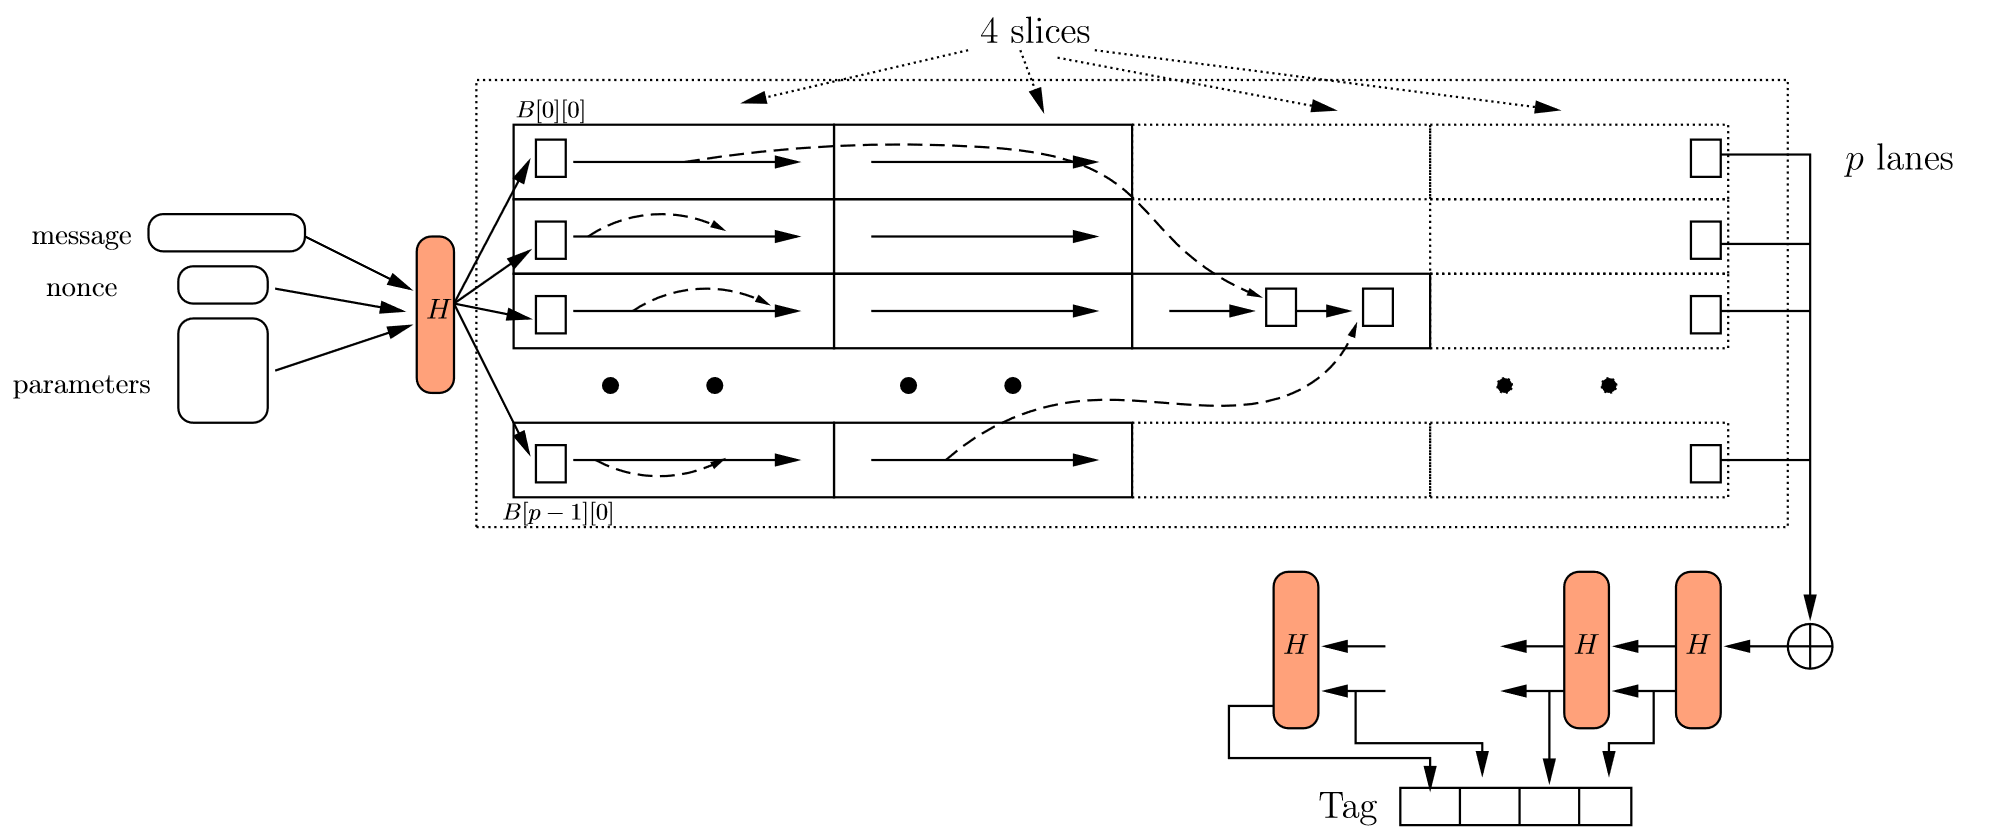
\includegraphics[scale=0.1]{assets/single-pass-argon2.png}
\caption{\textit{Single-pass} Argon2 com $p$ planos e 4 fatias. }\label{fig:argon2}
\end{figure}

Na figura \ref{fig:argon2} podemos ter uma visão geral do funcionamento do Argon2, 
neste exemplo existem $n$ planos e 4 fatias, recebe como input uma mensagem, \textit{Nonce} 
e os parâmetros descritos acima e como output, ou \textit{Tag}, temos uma string de $T$ 
bytes de comprimento. \cite{argon2spec}

Argon2d é otimizado para configurações onde o atacante não recebe
acesso regular à memória do sistema ou CPU, ou seja, não podem executar
ataques de canal com base nas informações de tempo, nem podem recuperar
a palavra-passe muito mais rápido usando a coleta de lixo. Essas configurações
são mais comuns para servidores de back-end e mineração de criptomoedas. Por
prática, são recomendadas as seguintes configurações:

\begin{itemize}
\item Mineração de criptomoedas, que leva 0,1 segundos num CPU de 2 GHz
usando 1 núcleo -- Argon2d com 2 pistas e 250 MB de RAM.
\end{itemize}

Argon2id é otimizado para configurações mais realistas, onde o
atacante pode possivelmente aceder a mesma máquina, usar o CPU ou montar
ataques de inicialização a frio. São recomendadas as seguintes configurações:

\begin{itemize}
\item Autenticação do servidor back-end, que leva 0,5 segundos em 2 GHz
CPU usando 4 núcleos -- Argon2id com 8 pistas e 4 GiB de RAM.
\item Derivação de chave para criptografia de disco rígido, que leva 3 segundos
uma CPU de 2 GHz usando 2 núcleos -- Argon2id com 4 pistas e 6 GiB de
RAM.
\item Autenticação do servidor front-end, que leva 0,5 segundos em 2 GHz
CPU usando 2 núcleos -- Argon2id com 4 pistas e 1 GiB de RAM.
\end{itemize} \cite{rfc9106}

\section{Performance do Algoritmo}

O tempo necessário para executar as operações de \textit{hash} na versão de consola são 
semelhantes às da versão PHP, com o aumento no tempo dependendo da memória 
adquirida para uso pelo algoritmo Argon2. Também é importante notar que a eficiência 
do algoritmo é amplamente influenciada pelo número de threads usadas. Com 1 GB de memória 
usada, seis iterações e um fio, o tempo gasto para realizar esta operação foi 
de quase 12 segundos. Com quatro threads, caiu quase para metade e com oito threads 
atingiu pouco mais de 4,5 segundos. Claro, o exemplo mencionado acima é apenas um exemplo 
limitante do algoritmo Argon2 no ambiente de produção, pois é cobrado com um pesado uso 
do poder do processador e da memória. O uso de memória de 16MB ou 32MB em três 
iterações e dois threads é a solução ideal em termos de tempo e uso de recursos 
de hardware. \cite{duka2020elliptic}

\section{Análise Criptográfica}

Os níveis de resistência de colisão e pré-imagem de Argon2 são equivalentes aos da função 
de \textit{hash} BLAKE2b subjacente. Para produzir uma colisão, são necessárias $2^{256}$ entradas. 
Para encontrar uma pré-imagem, $2^{512}$ entradas devem ser tentadas.
A segurança do KDF é determinada pelo comprimento da chave e pelo tamanho do estado interno 
da função \textit{hash} $h'$. Para distinguir o output do Argon2 com uma chave aleatória, são necessárias 
$(2^{128},2^{length(K)})$ chamadas mínimas para BLAKE2b.
O melhor ataque ao Argon2i de 1- e 2-passagens (v.1.3) é o ataque de baixo armazenamento 
de ~ \ cite {corrigan-gibbsB16}, que reduz o produto da área de tempo (usando o valor de 
memória de pico) pelo fator de 5. O melhor ataque para $T$-passagens ($T>2$) Argon2i é o 
ataque de troca de classificação, que reduz o produto da área de tempo pelo fator de 3.
O melhor ataque ao Argon2D $ T $  é o ataque de troca de classificação, que reduz 
o produto da área de tempo pelo fator 1.33. \cite{argon2spec}

Em termos de computação quântica, o algoritmo de Grover resolve essencialmente a tarefa de 
inversão da função. Se tivermos uma função $y = f(x)$ que pode ser avaliado num computador quântico, o algoritmo de 
Grover permite calcular $x$ quando dado $y$. Consequentemente, o algoritmo de Grover fornece amplas acelerações 
assintóticas para muitos tipos de ataques de força bruta à criptografia de chave simétrica, incluindo ataques 
de colisão e ataques de pré-imagem. \cite{bernstein2009post}

Existem alguns artigos publicados que têm foco em ataques ao algoritmo Argon2. 
O artigo de Boneh et al \cite{boneh2016balloon} mostra que é possível calcular uma função de passe 
de passagem única usando entre um quarto e um quinto do espaço desejado, sem penalidade 
de tempo, e calcular Argon2i com \textit{multi-pass} salvando um fator de $e \approx 2.72$ 
em espaço sem penalidade de tempo de computação. Este tipo de ataque foi corrigido na 
versão mais recente do Argon2, de acordo com os criadores \cite{argon2spec}, 
pelas experiências que fizeram, os resultados mostram que em 1-pass Argon2i, em média, $1/7$ 
da memória é usado. Como numa aplicação simples, em média, $1/2$ da memória é usado, 
a vantagem no produto da área de tempo é de cerca de $3.5$. Se for usado o valor da 
memória de pico nos cálculos da área de tempo, a vantagem seria de $5$ a $2.7$, respetivamente. 
A versão 1.3 do Argon2 substitui a operação de sobrescrever com o XOR. Isso fornece 
sobrecarga mínima sobre o desempenho: para os requisitos de memória de 8 MB e 
maior a diferença de desempenho é entre $5\%$ 3-Pass Argon2d v.1.2.1 em 1,8 GHz CPU 
com o Ubuntu é de $1.61$ ciclos por byte, enquanto para V.1.3 é $1.7$ ciclos por byte 
(ambos medidos para 2 GB de RAM, 4 threads). 

O artigo de Alwen-Blocki \cite{alwen2017towards} consiste em provar a efetividade do ataque de Alwen-Blocki, 
que na altura da sua criação afetava a revisão Argon2i-A (Versão 1.0), na revisão 
o Argon2i-B (Versão 1.3), com o objetivo de analisar a segurança dessa revisão em particular, 
tendo em consideração que o ataque seja realizado sob constrições de hardware realísticas. Este 
artigo é também o primeiro trabalho a analisar a segurança do Argon2i-B.
Conseguiram demonstrar que tal ataque, mesmo com tais constrições, é ainda possível de ser 
realizado na nova versão. Mesmo para definições de parâmetros pessimistas, o ataque 
conseguiu reduzir os custos por um fator de 2 usando apenas 1 GB de memória e que 
quando a largura de banda da memória limita o paralelismo, só era preciso ajustar 
os parâmetros de ataque em conformidade, sem afetar a qualidade de ataque. No entanto, 
o Argon2i-B demonstrou oferecer melhor resistência ao ataque do que Argon2i-A. 
O artigo também salienta que a redução dos custos de \textit{data-independent memory hard functions} (p. ex., por um fator de 10) podem 
aumentar a percentagem de palavras-passe comprometidas num ataque offline (por exemplo, por 
até $60\%$). Segundo a análise do artigo com os dados recolhidos foram mostrados os efeitos que vários 
parâmetros têm na memória consumo do ataque. Em particular, foram retiradas várias conclusões 
interessantes sobre o nível de segurança fornecido por essas funções.

\begin{itemize}
\item Para que o ataque Alwen-Blocki falhe contra parâmetros práticos de memória, Argon2i-B
deve ser instanciado com mais de 10 passagens na memória. A atual proposta do IRTF chama
mesmo apenas 6 passagens como a configuração ``paranoid'' recomendada.
\item De um modo mais geral, o processo de seleção de parâmetros na proposta é falho na medida em que
tende a produzir parâmetros para os quais o ataque é bem sucedido (mesmo sob condições realistas
restrições ao paralelismo).
\item A técnica de Corrigan-Gibs para melhorar a segurança também pode ser superada
pelo ataque Alwen-Blocki sob restrições de hardware realistas.
\item Numa nota positiva, tanto a segurança assintótica quanto a concreta do Argon2i-B parecem melhorar 
a de Argon2i-A.
\end{itemize}

O artigo de Chen et al \cite{chen2017investigation} teve como objetivo avaliar a qualidade do 
ataque de Alwen-Blocki. Conclui que o ataque apresenta uma ameaça teoricamente considerável 
para o Argon2, sendo uma ameaça preocupante a qualquer MHF com gráficos computacionais 
de indegredo fixo, praticamente falando ainda é uma melhoria em relação à disparidadeentre 
os ASIC e os computadores, em perfeita harmonia com a exigência não-memória de palavras-passe. 
No entanto, indicaram que o ataque optimizado por hardware não é generalizável a diferentes 
membros da família Argon2, sendo pouco provável que a maioria dos alvos utilize o mesmo 
membro da família Argon2. Também salientaram aência da compra de equipamentos generalizados 
sub-pares ou conjuntos diferentes de ASIC's para diferentes alvos, sendo uma limitação 
pragmática significante.

Segundo o artigo de \cite{Kodwani2021}, que faz uma análise sobre KDFs baseados em palavras-passe, 
devido às vulnerabilidades de ataques de colisão e $\delta$-cutback (sendo esta 
vulnerabilidade explicada da seguinte forma: um par de passwords que conduzem à mesma 
chave criptográfica pode ser encontrado fazendo $\delta$ menos chamadas para PBKDFs do 
que o ataque birthday aos PBKDFs) nos PBKDFs apresentados, a segurança efectiva 
de AES-128 baseado em palavra-passe está comprometida, e é equivalente para o 
DES de força bruta. As vulnerabilidades existem devido à utilização funções de 
\textit{hash} que funcionam de forma pseudo-random e a forma como as chaves criptográficas 
são derivadas do output da função pseudo-random. Tal como está agora,
um chamado esquema de encriptação computacionalmente seguro, tal como
AES, podem não ter qualquer ataque viável conhecido, mas se usado com
KDF como PBKDFs são propensas a ataques.

Traduzido com a versão gratuita do tradutor - www.DeepL.com/Translator

\section{Comparação com outros algoritmos existentes}

Existem vários algoritmos de \textit{hash} disponíveis para além do algoritmo em análise, Argon2, como por 
exemplo o MD5, SHA1, SHA256, PBKDF2, bcrypt, scrypt, ou simplesmente \textit{plaintext}. Com várias 
implementações de algoritmos de \textit{hash} pode-se tornar-se complicado perceber que 
diferenças existem entre os vários algoritmos, portanto nesta secção 
será realizada uma comparação dos algoritmos acima descritos, e outros, 
com o Argon2 e as suas derivações, Argon2i, Argon2d e Argon2id. 

\begin{table*}[hbt!]
\centering
\begin{adjustbox}{width=\textwidth}
\begin{tabular}{p{.18\textwidth}p{.22\textwidth}p{.2\textwidth}p{.2\textwidth}p{.2\textwidth}|l|l|l|l|l|}
    \hline
    Autor & Ano de publicação & Vantagens & Limitações \\
    \hline
    Belfedhal and Faraou \cite{belfedhal2015building} & 2015 & Fornece boas propriedades criptográficas tais como comportamento pseudo-aleatória e sensibilidade à entrada alterações. & Não foi testado contra ataques que são criptográficos em natureza, por exemplo, ataques de encontro no meio do caminho, colisão ou aniversário ataques. \\
    \hline
    Wang et al \cite{wang2015hash} & 2015 & Fornece uma saída variável. & Não foi testado contra ataques comuns, tais como colisão \\
    \hline
    Li et al \cite{li2016chaotic} & 2016 & Tem um bom desempenho estatístico e resistência à colisão. & Qualquer atacante pode lançar ataques de colisão exaustivos em a função porque o valor final do \textit{hash} é de 128 bits \\
    \hline
    Tur and Javure \cite{turvcanik2016hash} & 2016 &  & Ainda são necessários módulos extra para permitir que o sistema proposto possa ser utilizado como uma aplicação real.
    Não foi testado contra ataques que são de natureza criptográfica, por exemplo, ataques de encontro no meio, colisão ou aniversário. \\
    \hline
    Li and Liu \cite{li2017fast} & 2016 & A confusão e os bens de difusão de o algoritmo proposto é bom & Qualquer atacante pode lançar ataques de colisão exaustivos em a função porque o valor final do \textit{hash} é de 128 bits \\
    \hline
    Ahmad et al \cite{ahmad2017simple} & 2017 & Tem um grande desempenho estatístico. Pode gerar um valor \textit{hash} de comprimento 160,256 ou 512 bits. &  \\
    \hline
    Zhang et al \cite{zhang2017parallel} & 2017 & O algoritmo proposto satisfaz o requisito de desempenho estatístico & O algoritmo não é eficiente em termos de tempo para obter o valor de \textit{hash} \\
    \hline
\end{tabular}
\end{adjustbox}
\vspace{1em}
\caption{Comparação de variações de algoritmos de \textit{Hash}}
\label{hashcomptable}
\end{table*}
\cite{SHS2015}

A tabela \ref{hashcomptable} retirada do artigo de Maetouq et al \cite{maetouq2018comparison} 
contém uma comparação de vários algoritmos analisados e foi concluido que 
há vários tipos de algoritmos \textit{hash} utilizados para assegurar a integridade e 
autenticação de mensagens, alguns surgiram como padrão, tais como MD5, SHA-1, SHA-2 e SHA-3. 
Foi verificado neste artigo que a maioria deles ou são quebráveis, 
ou não são eficientes em termos de tempo. Além disso, este artigo discute outros 
algoritmos de \textit{hash} que foram apresentados por investigadores, mas a maioria deles 
não foram testados contra ataques que são de natureza criptográfica, tais como 
ataques de colisão. Portanto, pode concluir-se que uma função de \textit{hash} que seja 
eficiente e segura, e que cumpra requisitos de aplicação tais como integridade e 
autenticidade de dados, deve ser concebida e tornada numa prioridade.

\subsection{Utilização de \textit{plaintext}}

Começando com o mais óbvio, usar \textit{plaintext} (texto legível) para guardar informação delicada e 
portanto que deve ser escondida é o que deve ser evitado a todo o custo, pois 
qualquer pesquisa numa base de dados irá revelar todo o conteúdo de forma aberta 
a qualquer pessoa, daí a necessidade de usarmos algum algoritmo que torne esta 
informação encriptada. Ainda assim apesar da riqueza de métodos de criptografia 
existentes, algumas empresas ainda armazenam as palavras-passe em \textit{plaintext}, isso significa 
que qualquer pessoa com acesso pode ler todas as informações altamente confidenciais, 
como as palavras-passe, datas de nascimento e números de cartão de crédito. 
Se uma palavra-passe estiver armazenada em \textit{plaintext}, esta também pode ser rabiscada num bloco de notas e 
deixada na sala de espera para qualquer indivíduo mal itencionado ver. Bases de dados com 
palavras-passe em \textit{plaintext} tornam a contenção muito mais difícil porque o atacante compromete 
instantaneamente a segurança de todos os utilizadores do serviço web. Poderia ser 
considerado que um ataque directo num servidor é um evento extremamente improvável, 
mas incidentes recentes e repetidos em grande escala (afetando milhões de utilizadores) 
têm vindo a aumentar nos últimos anos \cite{ashley2022cyber} e principalmente com a 
guerra na Ucrânia temos visto isso a acontecer.

\subsection{Comparação com MD5}

Um dos algoritmos mais usados em bases de dados é o MD5, e é também um dos algoritmos mais velhos, 
criado em 1991, o algoritmo MD5 é uma extensão do algoritmo de \textit{hash} MD4. O MD5 é um pouco 
mais lento que o MD4, mas é mais "conservador" no design. Porque o MD4 foi criado para ser 
excepcionalmente rápido, é também muito susceptivel a ataques criptonalíticos bem-sucedidos. 
O MD5 recua um pouco, desistindo um pouco de velocidade por um maior probabilidade de segurança final. 
Este incorpora alguns sugestões feitas por vários revisores e contém otimizações adicionais. 
O algoritmo MD5-Digest é simples de implementar e produz como output um "fingerprint" ou \textit{hash} com um tamanho de 128 bits
de uma mensagem de comprimento arbitrário. É conjeturado que a dificuldade de apresentar duas mensagens 
ter o mesmo \textit{hash} está da ordem de $2^{64}$ operações, e que a dificuldade de apresentar qualquer mensagem 
tendo um dado \textit{hash} está na ordem de $2^{128}$ operações. \cite{rfc1321}

Por ser um algoritmo muito usado e pela sua idade, levaria a pensar que 
este seria um dos algoritmos mais seguros mas isto não se verifica.
Desde 1992, o MD5 foi extensivamente estudado e novos ataques criptográficos foram descobertos. 
Os algoritmos de \textit{hash} são desenhados para fornecer resistência de colisão, pré-imagem e segunda 
pré-imagem. O MD5 não é mais aceitável quando a resistência à colisão é necessária, 
como assinaturas digitais. Mas pode ser ainda usado para outros fins como o HMAC-MD5. 
As pseudo-colisões para a função de compactação do MD5 foram descritas pela primeira vez em 
1993 \cite{BoerCollisions}. Em 1996, \cite{DobbertinCryptanalysis} demonstrou um par de colisão 
para a função de compressão MD5 com um valor inicial escolhido. O primeiro artigo que demonstrou dois 
pares de colisão para MD5 foi publicado em 2004 \cite{Wang2004Collisions}. As técnicas de ataque detalhadas para o MD5 
foram publicadas em Eurocrypt 2005 \cite{WanginproceedingsHow}. Desde então, muitos resultados de pesquisa foram publicados 
para melhorar os ataques de colisão ao MD5. Os ataques apresentados em \cite{Klima2006Tunnels} podem encontrar 
colisão do MD5 em cerca de um minuto em um notebook padrão (Intel Pentium, 1,6 GHz). \cite{Stevens2007Collisions} 
afirma que leva 10 segundos ou menos em um pentium4 de 2,6 GHz para encontrar colisões. 
Em \cite{Stevens2007Collisions}, \cite{Stevens2007Chosen}, \cite{Stevens2009Short} e \cite{Stevens2012Chosen}, os ataques de colisão ao MD5 
foram aplicados com sucesso aos certificados X.509. Os ataque de colisão ao MD5 também podem ser 
aplicados a protocolos de autenticação challenge-and-response baseados em palavra-passe. \cite{rfc6151}

Para guardar palavras-passe em bases de dados o MD5 não é aconselhável há vários anos, o MD5 pode 
ter outros usos mas como é um algoritmo que usa apenas 128 bits para o \textit{hash} não consegue 
competir com o Argon2 que pode dar um output com um comprimento de $2^{32}$ bytes. Claro que 
pela diferença de anos em que estes algoritmos foram criados tem um impacto muito grande, pois 
desde 1992 houve uma evolução tecnológica muito grande.

\subsection{Comparação com SHA}

Os Secure Hash Algorithms são uma coleção de funções de \textit{hash} criptográfico divulgadas pelo 
National Institute of Standards and Technology (NIST) como Federal Information Processing 
Standard (FIPS) nos Estados Unidos. Incluem os algoritmos: 

\begin{itemize}
\item O SHA-1 é uma função de \textit{hash} de 160 bits que é semelhante ao método MD5. A National Security Agency 
(NSA) criou este algoritmo como parte do Digital Signature Algorithm. Depois de que as falhas 
criptográficas do SHA-1 foram encontradas, o padrão não foi mais autorizado para a maioria das 
aplicações criptográficas após 2010.
\item O SHA-2 consiste numa família de dois algoritmos de \textit{hash} semelhantes, SHA-256 e SHA-512, com tamanhos 
variados de blocos. O tamanho da palavra de SHA-256 e SHA-512 difere; O SHA-256 utiliza bits de 
32 bits e o SHA-512 usa palavras de 64 bits. Cada padrão também possui versões truncadas chamadas 
SHA-224, SHA-384, SHA-512/224 e SHA-512/256. A NSA também foi responsável por isto.
\item O SHA-3 é uma função de \textit{hash} que era anteriormente conhecida como Keccak sendo escolhida 
em 2012 após uma competição pública entre designers que não pertencem à NSA. Ele usa os mesmos 
comprimentos de \textit{hash} que o SHA-2 e possui uma estrutura interna diferente da restante da família SHA.
\end{itemize} \cite{SHA2022}

Estes algoritmos diferem mais significativamente no número de bits de segurança fornecidos para os dados 
que estão sendo \textit{hash} - isso está diretamente relacionado ao comprimento do resumo da mensagem. Quando um 
algoritmo de \textit{hash} seguro é usado em conjunto com outro algoritmo, pode haver requisitos especificados 
em outros lugares que exigem o uso de um algoritmo de \textit{hash} seguro com um certo número de bits de segurança. 
Por exemplo, se uma mensagem estiver sendo assinada com um algoritmo de assinatura digital que fornece 
128 bits de segurança, esse algoritmo de assinatura pode exigir o uso de um algoritmo de \textit{hash} seguro que 
também fornece 128 bits de segurança (por exemplo, SHA-256).
Na Tabela \ref{shatable} podemos ver algumas diferenças entre estes algoritmos.

\begin{table}[ht]
\centering
\begin{adjustbox}{width=0.5\textwidth}
\small
\begin{tabular}{|c|c|c|c|c|}
    \hline
    Algorithm & Message Size (bits) & Block Size (bits) & Word Size (bits) & Message Digest Size (bits) \\
    \hline
    SHA-1 & $< 2^{64}$ & 512 & 32 & 160 \\
    \hline
    SHA-224 & $< 2^{64}$ & 512 & 32 & 224 \\
    \hline
    SHA-256 & $< 2^{64}$ & 512 & 32 & 256 \\
    \hline
    SHA-384 & $< 2^{128}$ & 1024 & 64 & 384 \\
    \hline
    SHA-512 & $< 2^{128}$ & 1024 & 64 & 512 \\
    \hline
    SHA-512/224 & $< 2^{128}$ & 1024 & 64 & 224 \\
    \hline
    SHA-512/256 & $< 2^{128}$ & 1024 & 64 & 256 \\
    \hline
\end{tabular}
\end{adjustbox}
\vspace{1em}
\caption{Propriedades do Secure Hash Algorithm}
\label{shatable}
\end{table}
\cite{SHS2015}

\subsubsection{SHA-1}

O algoritmo SHA-1 é susceptível a ataques de colisão, pré-imagem e segunda pré-imagem. 
O primeiro ataque de colisão ao SHA-1 foi publicado no início de 2005 \cite{10100797835403057436}.
Este ataque descreveu um ataque teórico a uma versão do SHA-1
reduzido para 53 rodadas. Desde então, muitos novos métodos de análise foram desenvolvidos 
para melhorar o ataque apresentado em \cite{101007115352182}. No entanto, não há resultados publicados que
melhore os resultados encontrados em \cite{101007115352182}. \cite{manuel2011}, que é
A International Association for Cryptologic Research (IACR) Eprint
versão de \cite{manuel2011}, afirmou que o uso do método apresentado no
jornal, uma colisão de sha-1 completa pode ser encontrada em $2^{51}$ 
chamadas da função \textit{hash}. Os resultados da pesquisa conhecidos indicam que o SHA-1 não é tão
resistente à colisão como esperado. A força de segurança da colisão é
significativamente menor que uma função de \textit{hash} ideal (isto é, $2^{69}$ em comparação
a $2^{80}$). Não há ataques de pré-imagem ou segundos pré-imagem conhecidos que são
específicos para o algoritmo SHA-1 redondo completo. Kelsey e Schneier \cite{kelsey2005} descobriram um
resultado geral para todas as funções de \textit{hash} de Merkle-Damgaard
(que inclui SHA-1), encontrar uma segunda pré-imagem leva menos do que
$2^{n}$ cálculos. Quando $n = 160$, como é o caso do SHA-1, vai
Tome $2^{106}$ cálculos para encontrar uma segunda pré-imagem em um 60 byte
mensagem. Na ausência de ataques da rodada total, os criptografistas consideram
ataques reduzidos para pistas sobre a força de um algoritmo.
Ataques na rodada reduzida, onde o número de rodadas reduzidas não é mais
do que algumas menos que as rodadas completas, não demonstraram relacionar
para ataques completos. No entanto, o melhor ataque de rodada reduzida
indica uma certa margem de segurança. Por exemplo, se o mais conhecido
O ataque está em 60 em 80 rodadas, então o algoritmo tem cerca de 20
rodadas para resistir a ataques aprimorados. No entanto, a relação entre
o número de rodadas que um ataque pode alcançar e o número de rodadas
definido no algoritmo não é linear; não fornece um
prova matemática. \cite{rfc6194}

Como é o caso do MD5 e também pelo facto de que o SHA-1 é semelhante ao MD5, este algoritmo 
também não é recomendado para guardar palavras-passe, o NIST apenas recomenda o uso deste algoritmo 
para guardar informações não sensíveis, ou para verificar a integridade de informações. 
O Argon2 não é penalizado por estes ataques e como tal é mais seguro que o SHA-1.

\subsubsection{SHA-2}

A função SHA-2 é implementada em algumas aplicações e protocolos de segurança amplamente utilizados, 
incluindo TLS e SSL, PGP, SSH, S/MIME e IPSEC.
O SHA-256 é usado para autenticar pacotes de software Debian e no padrão de assinatura de 
mensagens DKIM; SHA-256 e SHA-512 são propostos para uso em DNSSEC. \cite{rfc5702}
Várias criptomoedas, incluindo Bitcoin, usam o SHA-256 para verificar transações e calcular o proof of work ou a 
prova de participação. \cite{sha256Bitcoin}
SHA-256 pode ser usado fazer o \textit{hash} de uma mensagem, M, com um comprimento de n bits, onde $0 \leq n < 2^{64}$, 
o algoritmo usa 1) um cronograma de mensagens de sessenta e quatro palavras de 32 bits, 
2) oito variáveis de trabalho de 32 bits cada e 3) um valor de \textit{hash} de oito palavras de 32 bits, 
o resultado final do SHA-256 é um \textit{hash} de 256 bits.
SHA-224 pode ser usado para \textit{hash} uma mensagem, m, tendo um comprimento de bits, onde $0 \leq n < 2^{64}$
A função é definida exatamente da mesma maneira que o SHA-256, com as duas seguintes exceções:
\begin{itemize}
\item O valor inicial do \textit{hash}, h (0), deve ser definido conforme uma certa especificação;
\item O resumo da mensagem de 224 bits é obtido cortando o valor final do \textit{hash}, $H(n)$, para os 224 
bits mais à esquerda.
\end{itemize}
SHA-512 pode ser usado para \textit{hash} uma mensagem, M, tendo um comprimento de bits, onde $0 \leq n < 2^{128}$, 
o algoritmo usa 1) um cronograma de mensagens de oitenta palavras de 64 bits, 2) oito variáveis 
de trabalho de 64 bits cada e 3) um valor de \textit{hash} de oito palavras de 64 bits. 
O resultado final do SHA-512 é um \textit{hash} de 512.
Os algoritmos SHA-384, SHA-512/224 e SHA-512/256 são definidos exatamente da mesma maneira que o SHA-512, 
mas com as exceções do SHA-224, substituindo os valores correspondentes do SHA-224 pelos seus respectivos valores. \cite{SHS2015}

Algumas das aplicações que usam \textit{hashes} criptográficos, como armazenamento de palavra-passe, são apenas 
minimamente afetados por um ataque de colisão. A construção de uma palavra-passe que funciona para uma 
determinada conta requer um ataque de pré-imagem, bem como acesso ao \textit{hash} da palavra-passe original 
(normalmente no arquivo de sombra) que pode ou não ser trivial. A criptografia de reversão de 
palavra-passe (por exemplo, para obter uma palavra-passe para tentar contra a conta de um usuário em outro lugar) 
não é possível pelos ataques. (No entanto, mesmo um \textit{hash} de palavra-passe segura não pode impedir ataques de 
força bruta em palavras-passe fracas.)
No caso de assinatura de documentos, um invasor não poderia simplesmente fingir uma assinatura de 
um documento existente - o invasor teria que produzir um par de documentos, um inócuo e um prejudicial, 
e fazer com que o detentor de chave privada assine o documento inócuo. Existem circunstâncias 
práticas em que isso é possível; Até o final de 2008, era possível criar certificados 
SSL forjados usando uma colisão MD5 que seria aceita por navegadores da Web amplamente utilizados.
O SHA-2 ainda pode ser considerado um algoritmo relativamente seguro, mas é inferior ao Argon2 
pois este oferece mais parâmetros de input para um \textit{hash} mais seguro.

\subsubsection{SHA-3}

O SHA-3 é o mais recente padrão Secure Hash Algorithm, lançada pelo NIST em 5 de agosto de 2015. 
Embora parte da mesma série de padrões, o SHA-3 é internamente diferente da estrutura do 
tipo MD5 de SHA-1 e SHA-2.
O SHA-3 é um subconjunto da família primitiva criptográfica mais ampla Keccak, criado por 
Guido Bertoni, Joan Daemen, Michaël Peeters e Gilles van Assche, construído a partir do Radiogatún. 
Os autores de Keccak propuseram usos adicionais para a função, ainda não (ainda) padronizados pelo 
NIST, incluindo um stream cipher, um sistema de criptografia autenticado, um esquema de \textit{hash} de 
"árvore" para \textit{hashes} mais rápidas em certas arquiteturas, e AEAD cifras Keyak e Ketje.
Keccak é baseado numa nova abordagem chamada sponge construction. A sponge construction 
é baseada numa ampla função aleatória ou permutação aleatória e permite a entrada ("absorção" 
na terminologia de esponja) qualquer quantidade de dados e saída ("espremendo" qualquer 
quantidade de dados, enquanto age como uma função pseudorandom com relação a todas as 
entradas anteriores, isso leva a uma grande flexibilidade.
Existe um resultado geral, o algoritmo de Grover, de que os computadores quânticos podem 
realizar um ataque de pré-imagem estruturado em $ \sqrt {2^{d}} = {2^{d/2}}$, enquanto um ataque clássico de 
força bruta de bruta precisa $2^{d}$. Um ataque estruturado de pré-imagem implica um segundo ataque de 
pré-imagem e, portanto, um ataque de colisão. Um computador quântico também pode realizar um 
ataque de aniversário, quebrar a resistência da colisão. \cite{SHA32022}

No artigo de Sumagita e Riadi \cite{sumagita2018analysis} foi usada a ferramenta \textit{Hashcat} 
que serve para obter um \textit{plaintext} de um \textit{hash} 
ou texto cifrado, no teste de força bruta, os dados obtidos da experência são o tempo necessário 
para obter um \textit{plaintext} usando como base um \textit{hash}, com o MD5 levou uma média de 54 segundos, 
enquanto o tempo necessário para o \textit{hash} com o SHA 512 levou uma média de 68 segundos. 

\subsection{Comparação com PBKDF2}

PBKDF2 aplica uma função pseudorandom para derivar chaves. A duração da chave 
derivada é essencialmente ilimitado (No entanto, o espaço de pesquisa efetivo 
máximo para a chave derivada pode ser limitada pela estrutura da função subjacente 
pseudorandom). Uma KDF produz uma chave derivada de uma chave base e
outros parâmetros. Numa KDF baseada em palavra-passe, a chave base é 
uma palavra-passe e os outros parâmetros são um valor de \textit{salt} e uma contagem de iteração.
A aplicação principal da derivação de chave baseada em palavra-passe. Outras aplicações são 
certamente possíveis, daí a definição independente destes funções. \cite{rfc2898}

PBKDF2 também pode ser usado com um \textit{password-based encryption scheme} (PBES), por exemplo, 
o PBES2 combina uma KDF baseada em palavra-passe com um esquema de criptografia 
subjacente. O comprimento da chave e quaisquer outros parâmetros para o esquema de criptografia 
subjacente dependem do esquema. Também pode ser usado como um esquema de autenticação de mensagem 
baseada em palavra-passe, um esquema de autenticação de mensagem consiste numa operação de geração de um 
\textit{Message Authentication Code} (MAC) e uma operação verificação do MAC, onde a operação de 
geração do MAC produz um MAC de uma mensagem sob uma chave, e a operação de verificação do MAC verifica o
código de autenticação da mensagem sob a mesma chave. Num esquema de autenticação de mensagem baseada 
em palavra-passe, a chave é uma palavra-passe. O PBMAC1 combina uma KDF baseada em palavra-passe com um
esquema de autenticação de mensagem subjacente. O comprimento da chave e quaisquer outros parâmetros 
subjacentes para o esquema de autenticação da mensagem depende do esquema. A criptografia baseada 
em palavra-passe é geralmente limitada na segurança que pode fornecer, principalmente para métodos como os 
PBES2 e PBMAC1 onde a pesquisa de palavra-passe offline é possível. Enquanto o uso de um \textit{salt} e uma contagem 
de iteração pode aumentar a complexidade do ataque, é essencial que as palavras-passe são bem selecionados 
e as diretrizes relevantes devem ser levadas em consideração. Também é importante que as palavras-passe sejam
bem protegido se são armazenadas. \cite{rfc8018}

As chaves derivadas em PBKDF2 também sofrem de não aleatoridade, embora as relações 
entre as chaves são um pouco mais complicadas. Seja s qualquer valor de \textit{salt}
e seja $c_1, c_2, c_3$ três contagens consecutivas de iteração. Para $i = 1, 2, 3$, defina
$y_i = F (p, s, c_i) = U_1 \oplus ... \oplus U_{ci}$. Então, temos $y_1 \oplus y_2 = U_{c2}$ e $y_2 \oplus y_3 = U_{c3}$.
Isso produz a seguinte relação entre as três chaves: $(y_2 \oplus y_3) = H_p (y_1 \oplus y_2)$,
onde $H_p()$ é a função subjacente HMAC.
Essa relação entre keys abre a porta para ataques de dicionário. O atacante simplesmente 
calcula a função HMAC $H_p (U_{c2})$ para todas as palavras-passe possíveis $P$, e a palavra-passe que 
fornece $H_p (U_{c2}) = U_{c3}$ é muito provável que seja a correta
palavra-passe usada no esquema. Uma vez que $P$ é conhecido, é fácil distinguir a
chave derivada de uma string aleatória. Observamos que a carga de trabalho do ataque acima 
é $| P W |$, não importa o que seja. Isso implica que a contagem de iteração não
adicione muita (ou qualquer) proteção no PBKDF2 contra ataques de dicionário. \cite{Yao2005Design}

\subsection{Comparação com bcrypt}

O bcrypt é um algoritmo de \textit{hash} criado por Niels Propos e David Mazières, 
baseado na cifra do Blowfish e apresentada na USENIX em 1999 \cite{bcryptspec}. Além de incorporar 
um \textit{salt} para proteger contra ataques que usam uma \textit{rainbow table}, o bcrypt é 
uma função adaptativa: com o tempo, a contagem de iteração pode ser aumentada para 
torná-la mais lenta, portanto permanece resistente a ataques de força bruta, 
mesmo com o aumento do poder de computação.
A função bcrypt é o algoritmo de \textit{hash} de palavra-passe padrão para o OpenBSD \cite{bcryptbsd} e foi o padrão 
para algumas distribuições Linux, como o SUSE Linux \cite{bcryptsuse}.
É importante observar que o bcrypt não é uma KDF. Por exemplo, não pode ser usado 
para extrair uma chave de 512 bits de uma palavra-passe. 
Ao mesmo tempo, algoritmos como PBKDF2, scrypt e Argon2 são KDFs baseadas em palavra-passe 
onde a saída é usada para fins de \textit{hash} de palavra-passe, em vez de apenas derivação de chave.
PBKDF2 é mais fraco que o bcrypt, o algoritmo de \textit{hash} SHA-2 geralmente usado não é memory-hard. 
O SHA2 foi criado para ser extremamente leve, para que possa ser executado 
em dispositivos computacionalmente fracos (por exemplo, cartões inteligentes) \cite{SHS2002}. 
Isso significa que o PBKDF2 é muito fraco para armazenamento de palavra-passe. Scrypt é mais fraco que 
o bcrypt para requisitos de memória inferior a 4 MB \cite{anthony2014why}.
O scrypt requer aproximadamente 1000 vezes a memória do bcrypt para obter um nível 
comparável de defesa contra ataques baseados em GPU (para armazenamento de palavra-passe). \cite{bcryptwiki}

O Argon2 é comparável com o bcrypt em tempos de execução inferiores a 1 segundo para autenticação 
de palavra-passe. Uma vantagem que o Argon2 tem em relação ao bcrypt é poder ser um KDF (baseado em palavra-passe), 
o Argon2d também pode ser usado para criptomoedas ou aplicações que requerem \textit{proof-of-work} pois 
é mais rápido que Argon2i e por sua vez bcrypt, mas também é relativamente mais inseguro.

\subsection{Comparação com BLAKE2}

A função \textit{hash} criptográfica BLAKE2 foi criada por Jean-
Philippe Aumasson, Samuel Neves, Zooko Wilcox-O'Hearn e Christian
Winnerlein. BLAKE2 vem em duas versões básicas:

\begin{itemize}
\item BLAKE2b (ou apenas BLAKE2) é otimizado para plataformas de 64 bits e
produz resumos de qualquer tamanho entre 1 e 64 bytes.
\item BLAKE2s é otimizado para plataformas de 8 a 32 bits e produz
\textit{digests} de qualquer tamanho entre 1 e 32 bytes.
\end{itemize}

BLAKE2 não requer uma construção especial "HMAC" (Código de autenticação de mensagem com \textit{hash})
para autenticação de mensagem com chave, pois possui uma chave integrada
mecanismo. A função \textit{hash} BLAKE2 pode ser usada por algoritmos de assinatura digital
e autenticação de mensagens e mecanismos de proteção de integridade em
aplicativos como Infraestrutura de Chave Pública (PKI),
protocolos de comunicação, armazenamento em nuvem, deteção de intrusão, forense
suítes e sistemas de controle de versão. A suíte BLAKE2 oferece uma alternativa mais eficiente ao US Secure
Algoritmos de \textit{hash} SHA e HMAC-SHA \cite{rfc6234}. BLAKE2s-128 é
especialmente adequado como uma substituição rápida e mais segura para
MD5 e HMAC-MD5 em aplicações legadas \cite{rfc6151}. \cite{rfc7693}

\section{Conclusão}

O Argon2 é um dos algoritmos de \textit{hash} mais seguros da atualidade, é inspirado nalguns 
algoritmos também considerados seguros até ao momento como o Bcrypt e Scrypt e por isso 
acaba por ser uma evolução lógica dos algoritmos de \textit{hash}, tira proveito do conhecimento 
adquirido sobre os algoritmos criados até ao momento do desenho do Argon2. Apenas uma versão do algoritmo tem 
vulnerabilidades que podem ser consideradas gravas, mas estas vulnerabilidades podem ser 
negadas como explicado na secção “Análise criptográfica”. Este algoritmo tem muitas 
vantagens, mas uma desvantagem que pode causar problemas nalgumas situações é o fato do 
algoritmo poder ser muito lento caso sejam modificados alguns parâmetros, é necessário 
criar um equilíbrio nestas situações entre segurança e tempo de execução. Apesar de ser 
um algoritmo seguro não tem muito suporte por parte de organizações ou individuos, como podemos
verificar pelo número de downloads deste algoritmo \cite{hashtrends}, e por exemplo as bases 
de dados mais usadas (MySQL ou MariaDB) suportam o MD5 ou SHA-2 mas não o Argon2.

\bibliographystyle{IEEEtran}
\bibliography{assets/references}

\end{document}
